\chapter{Boolean Retrieval}

\begin{multicols*}{2}

\noindent Information retrieval is \textit{finding material} (usually documents) of an \textit{unstructured nature} (usually text) that satisfies an information need from within \textit{large collections} (usually stored on computers)

\section{Term-document incidence}
\noindent Value 1 means the existence of a word in a specific document, value 0 otherwise. We treat each document as a boolean vector, and we just need to use boolean operation to answer query. 

\begin{center}
\begin{tabular}{ |c|c|c|c| } 
    \hline
     & Document A & DocumentB & Document C \\
    \hline 
    Antony & 1 & 1 & 0 \\ 
    Brutus & 1 & 1 & 0 \\
    Caesar & 1 & 1 & 0 \\
    Calpurnia & 0 & 1 & 0 \\ 
    \hline
\end{tabular}
\end{center}

\noindent However, the table / matrix above would be extremely sparse if we have more documents. For this reason, we would need inverted index.

\section{Inverted Index}
\noindent For each term, we store a list of all documents that contain the term. We use a variable-size postings list. The dictionary is lexically sorted. Document frequency for each term is stored.

\begin{center}
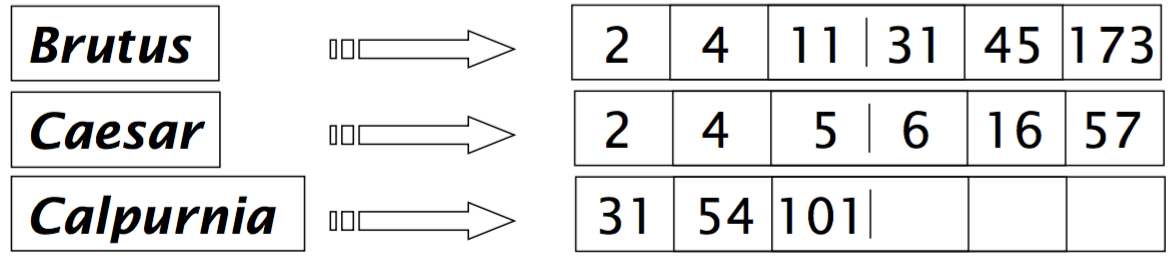
\includegraphics[width=8cm]{inverted-index}
\end{center}

\subsection{Query Processing: AND operation}
Locate two postings and merge the postings. The merging algorithm:
\begin{center}
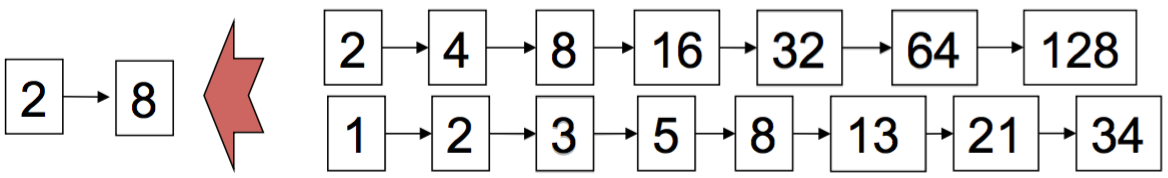
\includegraphics[width=8cm]{merging}
\end{center}

\section{Pros of Boolean Queries}
Pros: the retrieval is precise because it is either matches condition or not, it is the simplest model to build an IR system, works well when you know exactly what you are getting

\section{Query Optimisation}
We estimate the size of each OR operation by summing up the document frequency, estimate AND operation by taking the minimum document frequency. By processing query in order of increasing frequency, we can optimise the query. 

\section{Phrase Queries}
Answer queries such as ``Stanford University'' as a phrase. There are two ways to solve the problems: bi-word indexes and positional indexes. \\

\noindent Bi-word Indexes: Similar to inverted indexes, but the dictionary is bigram instead of unigram. However, the dictionary size grows larger. \\

\noindent Positional Indexes: the position for each term in each document. It is standardly used.
\begin{center}
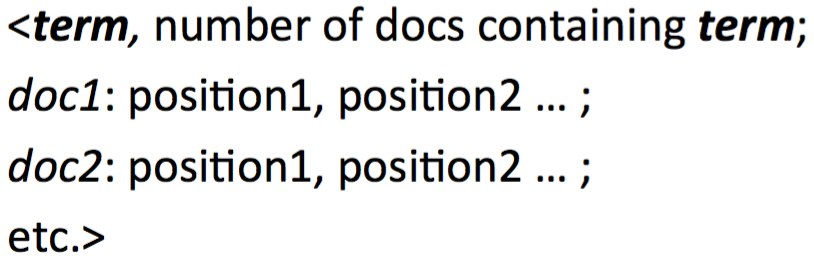
\includegraphics[width=8cm]{positional-index}
\end{center}

\section{Optimisation 1: Skip pointers}
\begin{center}
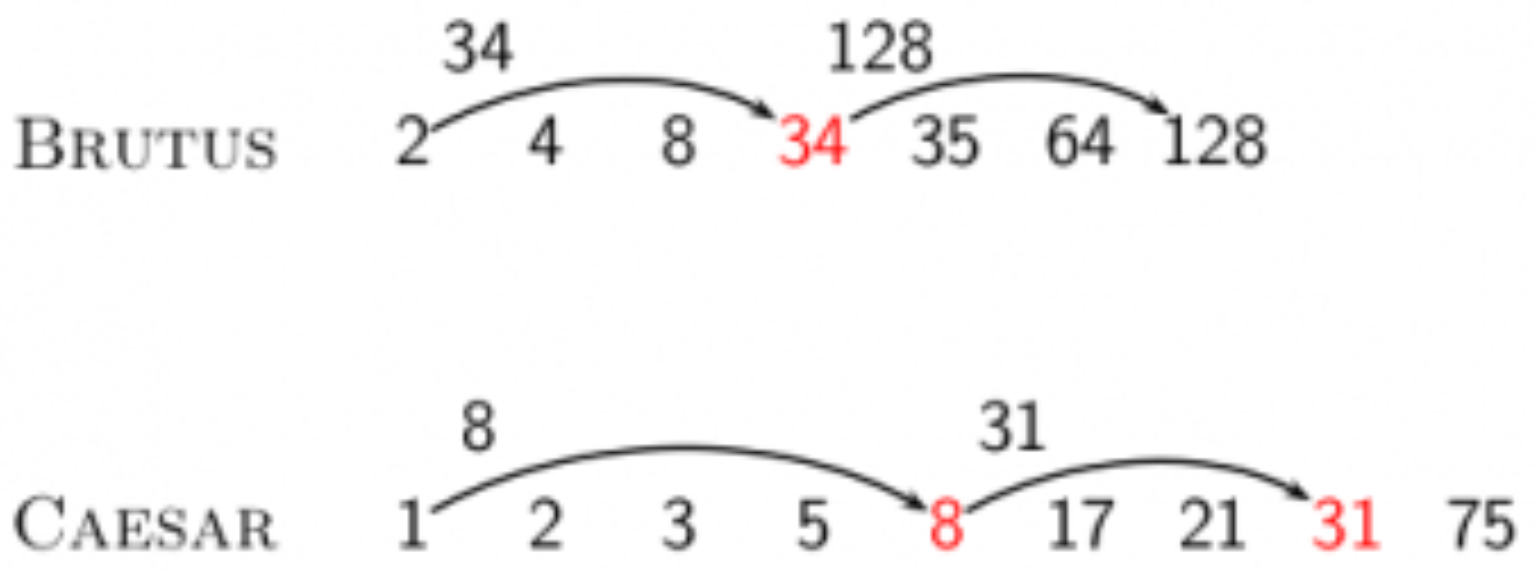
\includegraphics[width=8cm]{skip-pointer}
\end{center}

\section{Optimisation 2: Compression}
Motivation: less disk space, increase speed of data transfer from disk to memory

\subsection{Compress Dictionary}
We compress dictionary because searching begins with the dictionary. \\

\noindent Compression 1: Instead of storing terms as fixed width, we store dictionary as a long string of characters and use a term pointer to point to the start of a term.\\

\noindent Compression 2: Store pointers to every k-th term string, so we are not storing pointers to each term. However, we need to store extra term lengths for each term. (aka. Blocking)\\

\noindent Compression 3: Since sorted words commonly have long common prefix, we store the differences only. For example, ``automata, automate, automatic, automation'' will be stored as ``8automat*a1*e2*ic3*ion''. (aka. Front coding)

\subsection{Posting Compression}
Initially, we store a list of documents in increasing order. To compress posting, we can only store the gaps between each element. 

\section{Extra: Heaps’ Law}
$$M=kT^b$$

\noindent where:
\begin{equation*}
\begin{split}
    M: & \text{size of vocabulary} \\
    T: & \text{number of tokens}
\end{split}
\end{equation*}

\noindent Typically: 
$$30 \le k \le 100$$
$$b \approx 0.5$$

\section{Extra: Zipf’s Law}
The $i$-th most frequent term has frequency proportional to $1 / i$
\begin{center}
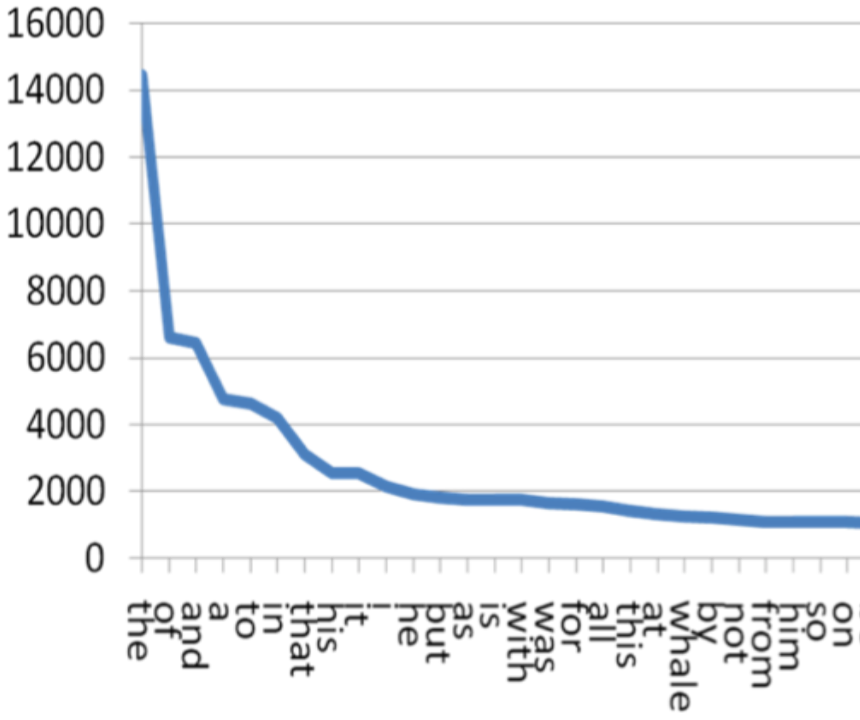
\includegraphics[width=8cm]{zipf-law}
\end{center}

\end{multicols*}